\newcommand{\RequiredPeers}{\ensuremath{N_\mathit{rs}}}

\chapter{Ouroboros Genesis}
\label{genesis}

\section{Introduction}

\subsection{Background: understanding the Longest Chain rule}
\label{genesis:background:longest-chain}

Recall the Praos chain selection rule:

\begin{definition}[Longest Chain Rule]
\label{longest-chain-rule}
A candidate chain is preferred over our current chain if
%
\begin{enumerate}
\item it is longer than our chain, and
\item the intersection point is no more than $k$ blocks away from our tip.
\end{enumerate}
\end{definition}

The purpose of chain selection is to resolve temporary forks that arise from the
normal operation of the protocol (such as when there are multiple leaders in a
single slot), and---importantly---to distinguish honest chains from chains
forged by malicious nodes. It is not a priori clear why choosing longer chains
over shorter chains would help distinguish malicious chains from honest chains:
why would an honest chain be longer?

Recall that the leadership schedule is based on stake: a node's probability of
being elected a leader in a given slot is proportional to their stake. By
assumption, the malicious nodes in the system together have less stake than the
honest nodes; security of the system as a whole critically depends on the
presence of this honest majority. This means that when a malicious node extends
the chain they can only produce a chain with relatively few filled slots: the
honest chain will be \emph{denser}. At least, this will be true near the
intersection point: as we get further away from that intersection point, the
malicious node can attempt to influence the leadership schedule for future slots
to their advantage.

The Praos security analysis \cite{cryptoeprint:2017:573} tells us that provided
all (honest) nodes are online all the time, they will all share the same chain,
except for blocks near the tips of those chains. Moreover, blocks with a slot
number ahead of the wall clock are considered invalid. This means that the only
way\footnote{The chain sync client does actually allow for some clock skew.
Headers that exceed the clock skew are however not included in chain selection.}
for one chain to be longer than another is by having more filled slots between
the tip of the shared prefix and ``now'': in other words, they must be
\emph{denser}.\footnote{A slightly subtle point arises from era transitions on
the chain that may change parameters such as the active slot coefficient,
allowing for denser chains after the transition. Although an adversary can
introduce such a transition on their own fork, such a transition would not take
effect until one stability window later, and so this won't affect the density
near the intersection point. Era transitions that are agreed on on the main
chain  benefit the honest parties and the adversary equally.}
%
\begin{center}
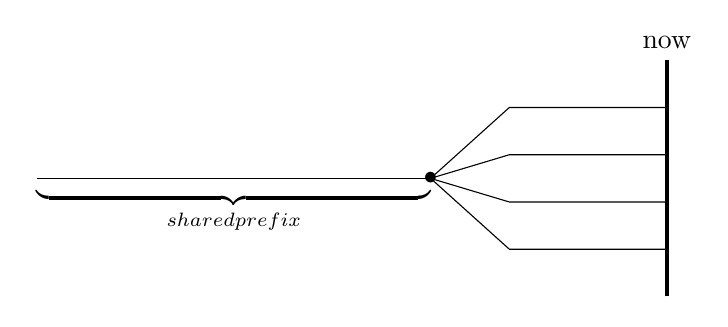
\begin{tikzpicture}
\draw (0,0) -- (5,0) coordinate(branch) node{$\bullet$} node[pos=0.5,below]{$\underbrace{\hspace{5cm}}_\text{shared prefix}$};
\draw (branch) -- ++(1,  0.9) -- ++(2,0);
\draw (branch) -- ++(1,  0.3) -- ++(2,0);
\draw (branch) -- ++(1, -0.3) -- ++(2,0);
\draw (branch) -- ++(1, -0.9) -- ++(2,0);
\draw [ultra thick] (8,-1.5) -- (8,1.5) node[above]{now};
\end{tikzpicture}
\end{center}
%
This motivates the first part of the Longest Chain rule: chain length is a
useful proxy for chain density, which in turn reflects honesty. The second part
of the rule---the intersection point is no more than $k$ blocks away from our
tip---is important because we can only meaningfully compare density \emph{near
  the intersection point}. As we get further away from the intersection point,
an adversary can start to influence the leadership schedule. This means that if
the adversary's chain forks off from the honest chain far back enough, they can
construct a chain that is longer than the honest chain. The Longest Chain rule
therefore restricts rollback, so that we will simply not even consider chains
that fork off that far back. We can still resolve minor forks that happen in the
honest chain during the normal operation of the protocol, because---so the
analysis guarantees---those will not be deeper than $k$ blocks.

\subsection{Nodes joining late}
\label{genesis:background:joining-late}

When new nodes join the network (or rejoin after having been offline for a
while), they don't have the advantage of having been online since the start of
the system, and have no sufficiently long prefix of the honest chain available.
As we saw at the end of \cref{genesis:background:longest-chain}, simply looking
at chain length is insufficient to distinguish the honest chain from malicious
chains: given enough time, an adversary can produce a chain that is longer than
the honest chain:
%
\begin{center}
\begin{tikzpicture}[yscale=0.5]
\draw (-2,0) node{$\bullet$} -- (0,0);
\draw (0,0) node{$\bullet$} -- (6,0) node{$\bullet$} node[right] {honest chain};
\draw (0,0) -- (0,-1) -- (8,-1) node{$\bullet$} node[right]{adversary's chain};
\path (0,0) -- (6,0) node[pos=0.5, above]{$\overbrace{\hspace{6cm}}^{\text{$\gg k$ blocks}}$};
\end{tikzpicture}
\end{center}
%
When a node's current chain is somewhere along that common prefix and uses the
longest chain rule, they will choose the adversary's chain rather than the
honest chain. Moreover, they will now be unable to switch to the honest chain,
because the intersection point with that chain is more than $k$ blocks ago. If a
node would get a ``leg up'' in the form of a reliable message telling which
chain to adopt when joining the network (such a message is known as a
``checkpoint'' in the consensus literature), the Praos rule from that point
forward would prevent them from (permanently) adopting the wrong chain, but
Praos cannot be used to help nodes ``bootstrap'' when they are behind.

So far we have just been discussing Praos as it is described in theory. The
situation in practice is worse. In the abstract models of the consensus
algorithm, it is assumed entire chains are being broadcast and validated. In
reality, chains are downloaded and validated one block at a time.
We therefore don't see a candidate chain's \emph{true} length; instead, the
length of a candidate we see depends on how much of that candidate's chain we
have downloaded\footnote{Even if nodes did report their ``true length'' we would
have no way of verifying this information until we have seen the entire chain,
so we can make no use of this information for the purpose of chain selection.}.
Defining chain selection in terms of chain length, where our \emph{perceived}
chain length depends on what we decide to download, is obviously rather
circular. In terms of the above discussion, it means that the adversary's chain
doesn't even need to be longer than the honest chain:
%
\begin{center}
\begin{tikzpicture}[yscale=0.5]
\draw (-2,0) node{$\bullet$} -- (0,0);
\draw (0,0) node{$\bullet$} -- (10,0) node{$\bullet$} node[right] {honest chain};
\draw
   (0,0)
  -- (0,-1)
  -- (4,-1)
    node{$\bullet$}
    node[right]{adversary's chain}
    node[pos=0.5, below]{$\underbrace{\hspace{4cm}}_{\text{$> k$ blocks}}$};
\end{tikzpicture}
\end{center}
%
If the adversary's chain contains more than $k$ blocks after the intersection
point, and we \emph{happen} to download that chain first, we would adopt it and
subsequently be unable to switch to the honest chain; after all, that would
involve a rollback of more than $k$ blocks, which the Praos rule forbids.

\clearpage

\subsection{The Density rule}
\label{genesis:background:density-rule}

It is therefore clear that we need a different chain selection rule so that
nodes can (re)join, and the Ouroboros Genesis paper \cite{cryptoeprint:2018:378}
proposes one, shown in \cref{genesis:maxvalid-bg}. In this chapter we will work
with a slightly simplified (though equivalent) form of this rule, which we will
term the Density Rule:
%
\begin{definition}[Density Rule]
A candidate chain is preferred over our current chain if it is denser
(contains more blocks) in a window of $s$ slots anchored at the intersection
between the two chains.
\end{definition}
%
(We will briefly discuss the differences between the rule in the paper and this
one in \cref{genesis:original}.) Technically speaking, $s$ is a
parameter of the rule, but the following default is a suitable choice both from
a chain security perspective and from an implementation perspective:\footnote{If
we change the epoch size, this value might have to be reconsidered, along with
the ledger's stability window.}

\begin{definition}[Genesis window size]
The genesis window size $s$ will be set to $s = 3k/f$.
\end{definition}

Unlike the Longest Chain rule, the Density rule does not impose a maximum
rollback. It does not need to, as it always considers density \emph{at the
intersection point}. This means that in a situation such as
%
\begin{center}
\begin{tikzpicture}[yscale=0.5]
\draw (-2,0) node{$\bullet$} -- (0,0);
\draw (0,0) node{$\bullet$} -- (10,0) node{$\bullet$} node[right] {honest chain};
\draw
     (0,0)
  -- (0,-1)
  -- (4,-1)
    node{$\bullet$} node[right]{adversary's chain}
    node[pos=0.5, below]{$\underbrace{\hspace{4cm}}_{\text{$> k$ blocks}}$};
\end{tikzpicture}
\end{center}
%
if we happen to see and adopt the adversary's chain first, we can still adopt
the honest chain (which will be denser at the intersection point, because of the
honest majority).This would however involve a rollback of more than $k$ blocks;
we will discuss how we can avoid such long rollbacks in
\cref{genesis:avoiding-long-rollbacks}.

\section{Properties of the Density rule}

In this section we will study the Density rule and prove some of its
properties. The improved understanding of the rule will be beneficial in the
remainder of this chapter.

\subsection{Equivalence to the Longest Chain rule}

For nodes that are up to date, the Density rule rule does not change how chain
selection works.

\begin{lemma}
\label{lemma:tip-density-is-chain-length}
When comparing two chains with an intersection that is at most $s$ slots away
from the two tips, the Density rule just prefers the longer chain.
\end{lemma}

\begin{proof}
The two chains share a common prefix, and differ only in the blocks
within the last $s$ slots:
%
\begin{center}
\begin{tikzpicture}[yscale=0.5]
\draw (0,0) -- (6,0) coordinate (I);
\draw (I) -- ++(1,1) -- ++(1.5,0);
\draw (I) -- ++(1,-1) -- ++ (2,0);
\draw [dashed]
    (I)
  -- ++(0, 1.5)
  -- ++(4, 0) node[pos=0.5,above]{$s$ slots}
  -- ++(0, -3)
  -- ++(-4, 0)
  -- cycle;
\end{tikzpicture}
\end{center}
%
Since the chain length in this case is simply the length of the length of the
common prefix plus the number of blocks in the window (i.e., their density),
the longer chain will also be denser in the window.

Just to be very explicit, \cref{lemma:tip-density-is-chain-length} does
\emph{not} hold when the intersection is more than $s$ slots away:
%
\begin{center}
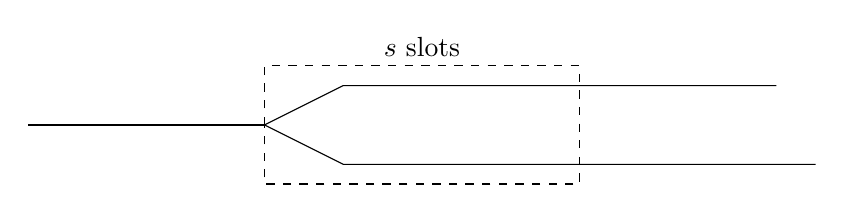
\begin{tikzpicture}[yscale=0.5]
\draw (0,0) -- (3,0) coordinate (I);
\draw (I) -- ++(1,1) -- ++(5.5,0);
\draw (I) -- ++(1,-1) -- ++ (6,0);
\draw [dashed]
    (I)
  -- ++(0, 1.5)
  -- ++(4, 0) node[pos=0.5,above]{$s$ slots}
  -- ++(0, -3)
  -- ++(-4, 0)
  -- cycle;
\end{tikzpicture}
\end{center}
%
In this case of course the longer chain may well not be denser in the window.
\end{proof}

\clearpage

\begin{lemma}[Rule Equivalence]
\label{lemma:rule-equivalence}
When comparing two chains with an intersection that is at most $k$ blocks away
from the two tips, the Density rule and the Longest Chain rule are equivalent.
\end{lemma}

\begin{proof}
First, observe that since the intersection is at most $k$ blocks away, the
maximum rollback condition of the Longest Chain rule is trivially satisfied.
Remains to show that the intersection is at most $s$ slots away, so that we can
apply \cref{lemma:tip-density-is-chain-length}. This is easiest to see by
contradiction: suppose the intersection is \emph{more} than $s$ slots away. Then
we would have a section on the chain which is more than $s$ slots long but
contains fewer than $k$ blocks; the Chain Growth analysis in
\cite{cryptoeprint:2017:573,cryptoeprint:2018:378} tells us that the probability
of this happening is negligibly small (provided $s$ is at least $3k/f$).
\end{proof}

\Cref{lemma:rule-equivalence} has a corollary that is of practical importance
for the consensus layer, as it re-establishes an invariant that we rely on
(\cref{never-shrink}):

\begin{lemma}
Alert nodes (that is, an honest node that has consistently been online)
will never have to switch to a shorter chain.
\end{lemma}

\begin{proof}
The Ouroboros Genesis analysis \cite{cryptoeprint:2018:378} tells us that
alert nodes will never have to roll back by more than $k$ blocks. In other
words, the intersection between their current chain and any chain they might
have to switch to will be at most $k$ blocks ago. The lemma now follows
from \cref{lemma:rule-equivalence}.
\end{proof}

\subsection{Honest versus adversarial blocks}

In this section we will consider what kinds of chains an adversary might try to
construct.

\begin{lemma}
\label{lemma:adversarial-before-k}
An adversary cannot forge a chain that forks off more than $k$ blocks from an
alert node's tip and is denser than the alert node's chain at the intersection
between the two chains.
\end{lemma}

\begin{proof}
This is an easy corollary of the Ouroboros Genesis analysis. If the adversary
would be able to construct such a chain, then by the Density rule the node
should switch to it. As mentioned above, however, the analysis tells us that
alert nodes never have to roll back more than $k$ blocks.
\end{proof}

\Cref{lemma:adversarial-before-k} has a useful specialization for chains that an
adversary might try to construct near the wallclock:

\begin{lemma}
\label{lemma:adversarial-within-s}
An adversary cannot forge a chain that satisfies all of the below:
%
\begin{itemize}
\item It forks off no more than $s$ slots from the wallclock.
\item If forks off more than $k$ blocks before the tip of an alert node.
\item It is longer than the alert node's current chain.
\end{itemize}
\end{lemma}

\begin{proof}
This example satisfies the first two criteria but not the third:
%
\begin{center}
\begin{tikzpicture}[yscale=0.75]
\draw
     (0,0)
  -- (6,0) coordinate (s-back) node{$\bullet$}
  -- (7,0) coordinate (k-back) node{$\bullet$};
\draw
     (k-back)
  -- ++(2, 1)
  -- ++(0, -2) node[pos=0.5,right=0.5]{honest chains}
  -- cycle;
\draw
     (s-back)
  -- ++(1, -2)
  -- ++(1, 0) node[right=1.5cm]{adversary's chain};
\path
     (k-back)
  -- ++(0, 1)
  -- ++(2, 0) node[pos=0.5,above]{$\overbrace{\hspace{2cm}}^{\text{$\le k$ blocks}}$};
\path
     (s-back)
  -- ++(0, 1.75)
  -- ++(3, 0) node[pos=0.5,above]{$\overbrace{\hspace{3cm}}^{\text{$\le s$ slots}}$};
\draw [very thick] (9, -2.5) -- (9, 2.5) node[above]{now};
\end{tikzpicture}
\end{center}
%
The intersection between the alert node's chain and the adversarial chain is
within $s$ slots from the wallclock. This means that density at the intersection
point is just chain length (\cref{lemma:tip-density-is-chain-length}), and
hence the property follows from \cref{lemma:adversarial-before-k}.
\end{proof}

\subsection{The original genesis rule}
\label{genesis:original}

The Density rule is simplification of the rule as presented in the paper
\cite{cryptoeprint:2018:378}.  The original rule is shown in
\cref{genesis:maxvalid-bg}, and paraphrased below:

\begin{definition}[Genesis chain selection rule, original version]
\label{genesis:originalrule}
A candidate chain is preferred over our current chain if

\begin{itemize}
\item The intersection between the candidate chain and our chain is \textbf{no
more than $k$} blocks back, and the candidate chain is strictly \textbf{longer}
than our chain.

\item If the intersection \emph{is} \textbf{more than $k$} blocks back, and the
candidate chain is \textbf{denser} (contains more blocks) than our chain in
a region of $s$ slots starting at the intersection.
\end{itemize}
\end{definition}

As we saw in \cref{lemma:rule-equivalence}, the Density rule is equivalent
to the Longest Chain rule if the intersection is within $k$ blocks, so the
original rule and the simplified form are in fact equivalent.

For completeness sake, we should note that this equivalence only holds for
suitable choice of $s$. If $s$ is much smaller (for example, the paper uses $s =
\frac{1}{4}(k/f)$ in some places), then we might have a situation such as the
following, where we have two chains $A$ and $B$; $A$ is denser than $B$ at the
intersection with $B$, but $B$ is longer:
%
\begin{center}
\begin{tikzpicture}
\path (0, 0) coordinate (tip) node{$\bullet$};
\draw (tip) -- ++(1.0,  0.5) -- ++(2.5, 0) coordinate(C1) node[right]{$A$};
\draw (tip) -- ++(1.0, -0.5) -- ++(3.5, 0) coordinate(C2) node[right]{$B$};
\draw [red, very thick] (tip) -- ++(1.0,  0.5) -- ++(2.0, 0);
\draw [dashed]
     (tip)
  -- ++(0, 0.75)
  -- ++(3, 0)
  -- ++(0, -1.5)
  -- ++(-3, 0) node[pos=0.5, below]{$\underbrace{\hspace{3cm}}_{\text{$s$ slots}}$}
  -- cycle;
\path (tip) -- (C1) node[pos=0.5, above=0.5cm]{$\overbrace{\hspace{3.5cm}}^{\text{fewer than $k$ blocks}}$};
\path (tip) -- (C2) node[pos=0.5, below=1.1cm]{$\underbrace{\hspace{4.5cm}}_{\text{more than $k$ blocks}}$};
\draw (tip) + (-3,0) node{$\bullet$} -- (tip);
\end{tikzpicture}
\end{center}
%
In this case, the original rule ends up preferring either $A$ or $B$ depending
on the order in which we consider them, whereas the Density Rule would simply
pick $A$. (As we we will in \cref{density-ordering-sensitivity}, however, the
Density rule is unfortunately not immune to order sensitivity either.)

\begin{figure}
\hrule

\textbf{Parameters} \\[0.5em]
\begin{tabular}{ll}
$C_\mathit{loc}$ & Current chain \\
$\mathcal{N} = \{C_1, \ldots, C_M\}$ & All possible chains (including our own) \\
$k$ & Security parameter (\cref{consensus:overview:k}) \\
$s$ & Genesis window size (Genesis rule specific parameter) \\
$f$ & Active slot coefficient (\cref{praos:f}) \\[1em]
\end{tabular}

\textbf{Algorithm}

\begin{lstlisting}[escapeinside={(*}{*)}, language={}, keywords={for,do,if,then,else,end,return}]
// Compare (*$C_\mathit{max}$*) to each (*$C_i \in \mathcal{N}$*)
Set (*$C_\mathit{max} \leftarrow C_\mathit{loc}$*)
for (*$i = 1$*) to (*$M$*) do
  if (*$(C_i \text{ forks from } C_\mathit{max} \text{ at most } k \text{ blocks})$*) then
    if (*$|C_i| > |C_\mathit{max}|$*) then // Condition A
      Set (*$C_\mathit{max} \leftarrow C_i$*).
  else
    Let (*$j \leftarrow \max \Bigl\{ j' \ge 0 \mathrel{\Bigl\lvert} C_\mathit{max} \text{ and } C_i \text{ have the same block in } \mathtt{sl}_{j'} \Bigr\} $*)
    if (*$|C_i[0 : j + s]| > |C_\mathit{max}[0 : j + s]|$*) then // Condition B
      Set (*$C_\mathit{max} \leftarrow C_i$*).
return (*$C_\mathit{max}$*)
\end{lstlisting}

\hrule
\caption{\label{genesis:maxvalid-bg}Algorithm \texttt{maxvalid-bg}}
\end{figure}

\section{Fragment selection}
\label{genesis:fragment-selection}

While the literature on Ouroboros compares entire chains, we will want to
compare \emph{fragments} of chains: if at all possible we would prefer not to
have to download and verify entire chains before we can make any decisions. As
we have discussed in \cref{genesis:background:joining-late}, comparing fragments
(prefixes) of chains using the Longest Chain rule does not actually make much
sense, but in this section we will see that the situation is fortunately much
better when we use the Density rule.

\begin{definition}[Preferred fragment]
Let $\mathcal{S}$ be set of chain fragments, all anchored at the same point
(that is, the fragments share a common ancestor), corresponding to some set of
chains $\mathcal{C}$. Then $A$ is a preferred fragment in $\mathcal{S}$ if and
only if $A$ is a fragment of a preferred chain in $\mathcal{C}$.
\end{definition}

We will now establish the (necessary and sufficient) condition for fragment
preference to be decidable. First, if we have to choose between two chains, we
must see enough of those chains to do a density comparison.

\pagebreak

\begin{definition}[Known density]
We say that a chain fragment has a \emph{known density} at some point $p$
if either of the following conditions hold:

\begin{enumerate}
\item The fragment contains a block after at least $s$ slots:
\begin{center}
\begin{tikzpicture}[yscale=0.75]
\path (0,0) -- (9,0); % adjust bounding box
\path (0,0) -- (1,0) node[pos=0.5]{$\cdots$};
\draw
     (1,0)
  -- (3,0)   node{$\bullet$} node[above left]{$p$} coordinate(p)
  -- (3.5,0) node{$\bullet$}
  -- (4,0);
\path
     (4,0)
  -- (5,0) node[pos=0.5]{$\cdots$};
\draw
     (5,0)
  -- (5,0) node{$\bullet$}
  -- (6,0) node{$\bullet$}
  -- (7,0) node[red]{$\bullet$}
  -- (8,0) node[right]{$\cdots$};
\draw [dashed]
     (p)
  -- ++(0, 1)
  -- ++(3.5, 0) node[pos=0.5,above]{$s$ slots}
  -- ++(0, -2)
  -- ++(-3.5, 0)
  -- cycle;
\end{tikzpicture}
\end{center}

\item The chain (not just the fragment\footnote{We can distinguish between these
two cases because nodes report the tip of their chain as part of the chain sync
protocol, independent from the headers that we have downloaded from those
nodes.}) terminates within the window:
\begin{center}
\begin{tikzpicture}[yscale=0.75]
\path (0,0) -- (9,0); % adjust bounding box
\path (0,0) -- (1,0) node[pos=0.5]{$\cdots$};
\draw
     (1,0)
  -- (3,0)   node{$\bullet$} node[above left]{$p$} coordinate(p)
  -- (3.5,0) node{$\bullet$}
  -- (4,0);
\path
     (4,0)
  -- (5,0) node[pos=0.5]{$\cdots$};
\draw
     (5,0)
  -- (6,0) node[red]{$\bullet$};
\draw [dashed]
     (p)
  -- ++(0, 1)
  -- ++(3.5, 0) node[pos=0.5,above]{$s$ slots}
  -- ++(0, -2)
  -- ++(-3.5, 0)
  -- cycle;
\end{tikzpicture}
\end{center}
\end{enumerate}
\end{definition}

\begin{definition}[Look-ahead closure]
\label{lookahead-closure}
Let $\mathcal{S}$ be a set of chain fragments all anchored at the same point. We
say that $\mathcal{S}$ is \emph{look-ahead closed} if whenever there are two
fragments $A, B \in \mathcal{S}$, the densities of $A$ and $B$ are known at
their intersection.
\end{definition}

\begin{lemma}[Look-ahead closure is sufficient for fragment selection]
\label{lemma:fragment-selection}
Let $\mathcal{S}$ be a look-ahead closed set of chain fragments. Then
we can always choose a preferred fragment in $\mathcal{S}$.
\end{lemma}

\begin{proof}[Proof (sketch)]
In order to be able to pick a chain, we need to resolve forks. In order to
resolve forks using the Density Rule, we need to know the density, but that
is precisely what is guaranteed by look-ahead closure.
\end{proof}

\pagebreak

\Cref{lemma:fragment-selection} is relevant because it reflects how the
consensus layer uses chain selection:

\begin{enumerate}
\item We maintain a fragment of the chain for each upstream peer we track
(\cref{chainsyncclient}). The block fetch client
(\cref{chainsyncclient:plausiblecandidates}) then picks a preferred fragment and
downloads that.
\item When the chain database needs to construct the current chain
(\cref{chainsel}), it constructs a set of chain fragments through the volatile
DB, all anchored at the tip of the immutable database, picks a preferred
fragment, and adopts that as the node's current chain.
\end{enumerate}

However, \cref{lemma:fragment-selection} is less useful than it might seem:
the look-ahead closure requirement means that in the worst case, we still need
to see entire chains before we can make a decision: every new intersection point
requires us to see $s$ more slots:
%
\begin{center}
\begin{tikzpicture}[yscale=0.5]
\path (0,0) coordinate(I);
%
\node at (I) {$\bullet$};
\draw (I) -- ++(2.5, 0);
\draw (I) -- ++(1,-1) -- ++(0.5,0) coordinate(A) -- ++(2,0);
\draw [dashed]
     (I)
  -- ++(0,0.25)
  -- ++(2,0)
  -- ++(0,-1.5)
  -- ++(-2,0) node[pos=0.5,below]{$\underbrace{\hspace{2cm}}_\text{$s$ slots}$}
  -- cycle;
%
\node at (A) {$\bullet$};
\draw (A) -- ++(2.5, 0);
\draw (A) -- ++(1,-1) -- ++(0.5,0) coordinate(B) -- ++(2,0);
\draw [dashed]
     (A)
  -- ++(0,0.25)
  -- ++(2,0)
  -- ++(0,-1.5)
  -- ++(-2,0) node[pos=0.5,below]{$\underbrace{\hspace{2cm}}_\text{$s$ slots}$}
  -- cycle;
%
\node at (B) {$\bullet$};
\draw (B) -- ++(2.5, 0);
\draw (B) -- ++(1,-1) -- ++(0.5,0) coordinate(C) -- ++(2,0) node[above=0.5cm, right]{$\cdots$};
\draw [dashed]
     (B)
  -- ++(0,0.25)
  -- ++(2,0)
  -- ++(0,-1.5)
  -- ++(-2,0) node[pos=0.5,below]{$\underbrace{\hspace{2cm}}_\text{$s$ slots}$}
  -- cycle;
\end{tikzpicture}
\end{center}
%
Moreover, due to the header/body split
(\cref{nonfunctional:network:headerbody}), when we are tracking the headers from
an upstream peer, we cannot (easily) verify headers that are more than $3k/f$
slots away from the intersection between our chain and their chain (see also
\cref{low-density}). In the next section we will therefore consider how we can
drop the look-ahead closure requirement.

In case it is not obvious why we must only compare density at intersection
points, in the remainder of this section we will consider an example that will
hopefully clarify it. Suppose a malicious node with some stake intentionally
skips their slot, after which the chain continues to grow as normal:
%
\begin{center}
\begin{tikzpicture}
\draw
       (0,0) node{$\bullet$}
  -- ++(1,0) node{$\bullet$}
  -- ++(1,0) node{$\bullet$}
  -- ++(1,0) node{$\bullet$}
  -- ++(1,0) node[above]{$\times$}
  -- ++(1,0) node{$\bullet$}
  -- ++(1,0) node{$\bullet$}
  -- ++(1,0) node{$\bullet$};
\end{tikzpicture}
\end{center}
%
It is now trivial for the adversary to create an alternative chain that
\emph{does} have a block in that slot; if other nodes switch to the denser chain
the moment they see a window of $s$ slots that is denser, they would adopt the
adversary's chain; after all, it has one more block in the window than the
honest chain does:
%
\begin{center}
\begin{tikzpicture}[yscale=0.5]
\draw
       (0,0) node{$\bullet$}
  -- ++(1,0) node{$\bullet$} coordinate(s-anchor)
  -- ++(1,0) node{$\bullet$}
  -- ++(1,0) node{$\bullet$} coordinate(branch)
  -- ++(1,0) node[above]{$\times$}
  -- ++(1,0) node{$\bullet$}
  -- ++(1,0) node{$\bullet$}
  -- ++(1,0) node{$\bullet$};
\draw
       (branch)
  -- ++(1, -1) node{$\bullet$}
  -- ++(3,  0) node{$\bullet$};
\draw [dashed]
     (s-anchor)
  -- ++(0,1)
  -- ++(3.5,0)
  -- ++(0,-2.5)
  -- ++(-3.5,0) node[below, pos=0.5]{$\underbrace{\hspace{3.5cm}}_{\text{$s$ slots}}$}
  -- cycle;
\end{tikzpicture}
\end{center}
%
Instead, we must wait until we make such a comparison until we have reached
the intersection point:
%
\begin{center}
\begin{tikzpicture}[yscale=0.5]
\draw
       (0,0) node{$\bullet$}
  -- ++(1,0) node{$\bullet$}
  -- ++(1,0) node{$\bullet$}
  -- ++(1,0) node{$\bullet$} coordinate(branch)
  -- ++(1,0) node[above]{$\times$}
  -- ++(1,0) node{$\bullet$}
  -- ++(1,0) node{$\bullet$}
  -- ++(1,0) node{$\bullet$};
\draw
       (branch)
  -- ++(1, -1) node{$\bullet$}
  -- ++(3,  0) node{$\bullet$};
\draw [dashed]
     (branch)
  -- ++(0,1)
  -- ++(3.5,0)
  -- ++(0,-2.5)
  -- ++(-3.5,0) node[below, pos=0.5]{$\underbrace{\hspace{3.5cm}}_{\text{$s$ slots}}$}
  -- cycle;
\end{tikzpicture}
\end{center}
%
Since the adversary does not have sufficient stake, their chain will be less
dense and we will therefore not select it. If the adversary creates another fork
earlier on the chain, then we will resolve that fork when we encounter it using
a window of $s$ slots \emph{anchored at that fork}, and then later resolve the
second fork using a \emph{different} window of $s$ slots, anchored at the second
fork:
%
\begin{center}
\begin{tikzpicture}[yscale=0.5]
\draw
       (0,0) node{$\bullet$}
  -- ++(1,0) node{$\bullet$} coordinate(s-anchor)
  -- ++(1,0) node{$\bullet$}
  -- ++(1,0) node{$\bullet$} coordinate(branch)
  -- ++(1,0) node[above]{$\times$}
  -- ++(1,0) node{$\bullet$}
  -- ++(1,0) node{$\bullet$}
  -- ++(1,0) node{$\bullet$};
\draw
       (branch)
  -- ++(1, -1) node{$\bullet$}
  -- ++(3,  0) node{$\bullet$};
\draw
       (s-anchor)
  -- ++(1, -1) node{$\bullet$};
\draw [dashed]
     (s-anchor)
  -- ++(0,1)
  -- ++(3.5,0)
  -- ++(0,-2.5)
  -- ++(-3.5,0) node[below, pos=0.5]{$\underbrace{\hspace{3.5cm}}_{\text{$s$ slots}}$}
  -- cycle;
\draw [dotted]
     (branch) ++ (0, 0.1)
  -- ++(0,1)
  -- ++(3.5,0)  node[above, pos=0.5]{$\overbrace{\hspace{3.5cm}}^{\text{$s$ slots}}$}
  -- ++(0,-2.5)
  -- ++(-3.5,0)
  -- cycle;
\end{tikzpicture}
\end{center}

\pagebreak

\section{Prefix selection}
\label{genesis:prefix-selection}

\subsection{Preferred prefix}

When a set $\mathcal{S}$ of chain fragments is not look-ahead closed, we may
not be able to pick a best fragment. For example, in
%
\begin{equation*}
\mathcal{S} = \left\{ \;
\begin{tikzpicture}[baseline=0pt, xscale=0.5,yscale=0.5]
\draw [very thick, red] (-2,0) -- (0,0);
\draw (0,0) -- (1, 1) -- (6,  1) node[right]{$A$};
\draw (0,0) -- (1,-1) -- (7, -1) node[right]{$B$};
\draw [dashed] (-2,0) -- ++(0,1.5) -- ++(5,0) node[pos=0.5,above]{$\overbrace{\hspace{2cm}}^\text{$s$ slots}$} -- ++(0,-3) -- ++(-5,0) -- cycle;
\end{tikzpicture}
\right\}
\end{equation*}
%
we cannot choose between $A$ and $B$; what we \emph{can} say however is that no
matter which of $A$ and $B$ turns out to be the better fragment, the common
prefix of $A$ and $B$ (shown in red) will definitely be a prefix of that
fragment. This example provides the intuition for the definition of a preferred
prefix:

\begin{definition}[Preferred prefix]
Given a set $\mathcal{S}$ of chain fragments, all anchored at the same point, a
preferred prefix is a prefix $\Pi$ of one of the fragments in $\mathcal{S}$,
such that $\Pi$ is guaranteed to be a prefix of a preferred fragment in the
lookahead-closure of $\mathcal{S}$.
\end{definition}

In other words, we may not be able to pick the best fragment out of
$\mathcal{S}$, but we \emph{can} pick a prefix which is guaranteed to be a
prefix of whatever turns out to be the best fragment. Obviously, the empty
fragment is always a valid choice, albeit not a particularly helpful one.
Ideally, we would choose the \emph{longest} preferred prefix. Fortunately,
constructing such a prefix is not difficult.

\subsection{Algorithm}

We will now consider how we can choose the longest preferred prefix.

\begin{definition}[Prefix selection]
\label{prefix-selection}
Let $\mathcal{S}$ be a set of chain fragments all anchored at the same point $a$,
such that all fragments have known density at point $a$. Then we can construct
the longest preferred prefix in two steps:
%
\begin{enumerate}
\item \emph{Resolve initial fork.}
Suppose $\mathcal{S}$ looks like this:
%
\begin{center}
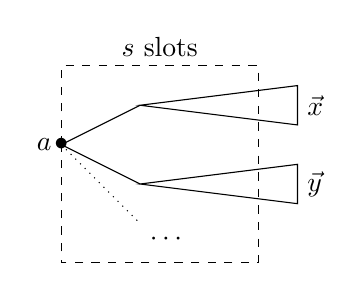
\begin{tikzpicture}
\node at (0,0) [left] {$a$};
\node at (0,0) {$\bullet$};
%
\draw (0,0) -- (1, 0.5) coordinate(x);
\draw (0,0) -- (1,-0.5) coordinate(y);
\draw [dotted] (0,0) -- (1,-1) node[below right]{$\cdots$};
%
\draw (x) -- ++(2,  0.25) -- ++(0, -0.5) node[pos=0.5,right]{$\vec{x}$} -- cycle;
\draw (y) -- ++(2,  0.25) -- ++(0, -0.5) node[pos=0.5,right]{$\vec{y}$} -- cycle;
%
\draw [dashed]
     (0,0)
  -- ++(0, 1)
  -- ++(2.5, 0) node[pos=0.5,above]{$s$ slots}
  -- ++(0, -2.5)
  -- ++(-2.5, 0)
  -- cycle;
\end{tikzpicture}
\end{center}
%
where (without loss of generality) the common prefixes are non-empty. Suppose
one of the $\vec{x}$ has the highest density\footnote{ If two fragments in
different forks have  have exactly the same density, we need a tie-breaker in
order to be able to make progress. The genesis paper does not prefer either
chain in such a scenario, switching only if another chain is strictly denser. We
can therefore follow suit, and just focus on one of the two chains arbitrarily.}
at point $a$; let's call it $x_i$. That means if we ever were to adopt any of
the $\vec{y}, \ldots$, and then compared our chain to $x_i$, we would find that
$x_i$ is denser at the intersection point (which is precisely what we are
comparing in this window here), and therefore switch to it. This means we can
focus our attention on the $\vec{x}$. (Unfortunately\todo{TODO}, the existing
density rule does not always pick a unique best chain, so we cannot prove this
algorithm correct. See \cref{density-ordering-sensitivity}.)

\item \emph{Adopt common prefix.}
Most of the time, the density of the $\vec{x}$ will yet not be known. This means
we do not yet know which $x_i$ will turn out to be the best, but we \emph{do}
know that whichever it turns out to be, it will have the common prefix from $a$
to $b$, so we choose this as the longest preferred prefix:

\begin{center}
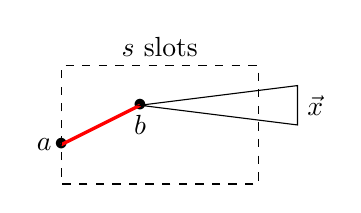
\begin{tikzpicture}
\path (0,0)   node{$\bullet$} node[left]{$a$};
\path (1,0.5) node{$\bullet$} node[below]{$b$};
%
\draw [very thick, red] (0,0) -- (1, 0.5) coordinate(x);
%
\draw (x) -- ++(2,  0.25) -- ++(0, -0.5) node[pos=0.5,right]{$\vec{x}$} -- cycle;
%
\draw [dashed]
     (0,0)
  -- ++(0, 1)
  -- ++(2.5, 0) node[pos=0.5,above]{$s$ slots}
  -- ++(0, -1.5)
  -- ++(-2.5, 0)
  -- cycle;
\end{tikzpicture}
\end{center}
%
One useful special case is when all of the $\vec{x}$ terminate within the
window. In this case, their density \emph{is} known, and we can just pick the
densest fragment as the preferred prefix; the preferred prefix is then in fact
the preferred fragment.
\end{enumerate}
\end{definition}

Prefix selection fits very naturally with the needs of the consensus layer
(\emph{cf.} the description of how consensus uses fragment selection in
\cref{genesis:fragment-selection}):
%
\begin{enumerate}
\item When blockfetch applies prefix selection to the set of fragments of
the upstream peers we are tracking, the computed prefix is precisely the set
of blocks that blockfetch should download.
\item When the chain database applies prefix selection to the set of fragments
through the volatile database, the computed prefix is precisely the chain that
we should adopt as the node's current chain.
\end{enumerate}

\begin{lemma}
If the intersection point between the chains of our upstream peers is at most
$k$ blocks away from their tips, prefix selection will choose the longest chain.
\end{lemma}

\begin{proof}[Proof (sketch)]
The proof is very similar to the proof of \cref{lemma:rule-equivalence}.
If the intersection is at most $k$ blocks away, it will be less than $s$ slots
away; therefore prefix selection will be able to see the chains to their tip,
the density of all chains will be known, and the densest fragment equals the
longest one.
\end{proof}

\subsection{Prefix selection on headers}

When the chain sync client is dedicing which of the chains of its upstream peers
to download, it does so based on chains of \emph{headers}. It does not download
block bodies and so cannot verify them. As such, it is basing its decisions
based on header validity \emph{only}.  However, this is then only used to tell
the block fetch client which blocks to \emph{download}
(\cref{chainsyncclient:plausiblecandidates}); it does not necessarily mean that
those blocks will be \emph{adopted}. When the chain database performs chain
selection (\cref{chainsel}), it will verify the blocks and discard any that turn
out to be invalid. If any blocks \emph{are} invalid, then the chain sync client
will disconnect from the nodes that provided them, which in turn may change
which prefix is chosen by prefix selection.

Indeed, the only reason to even validate headers at all is to avoid a denial
of service attack where an adversary might cause us to waste resources.
It may be worth reconsidering this risk, and balancing it against the costs
for the implementation; the only reason we need forecasting, and a special
treatment of low density chains (\cref{low-density}) is that we insist we want
to validate headers independent from blocks.

\subsection{Known density}

\Cref{prefix-selection} requires known density at the anchor $a$ of the set, so
that it can resolve the initial fork. This means we have to wait until
we have downloaded enough headers from each peer: the last header we downloaded
must either be outside the $s$ window, or else it must be the last header on that
peer's chain (in which case the peer will tell us so). If a peer tells us they have
more headers but then do not provide them, we should disconnect from them
after some time-out to avoid a potential denial of service attack.

Note that if that last header is \emph{not} the last header on a peer's chain,
we will not be able to validate it: since it is more than $s$ slots away from
the anchor point (and we only have a ledger state at the anchor point), it falls
outside the ledger's forecast range. However, this does not matter: the presence
of this header only tells us that we have seen everything we need to see to
compute the density within the window; an invalid header after that window
cannot increase the density \emph{within} the window.

\pagebreak

We can make two useful exceptions to the known density requirement:

\begin{enumerate}
\item If there \emph{is} no initial fork, we do not need to know the density at
all and can go straight to step (2). This will allow a node to sync faster:
consider a new node that is joining the network. In most cases, all of the
node's upstream peers will report the \emph{same} blocks for all but the last
few blocks on the chain. Since there is no fork to resolve, we can start
adopting blocks the moment we see them.

\item When we say that the density is \emph{known}, we mean that we have seen
the last required header and validated it. However, consider what happens when
the node is up to date, and a new block is produced (by some other node).
Strictly speaking we must now wait for \emph{all} peers to have provided us with
this header, and have validated all those headers, before we would consider the
density to be known and prefix selection can make progress. This is however
unnecessary: when node $A$ provides us with a header, and then node $B$ reports
the exact same tip, we know that node $B$'s density cannot exceed node $A$s, and
so we can go ahead and select node $A$'s chain.
\end{enumerate}

\begin{figure}[p]
\hrule
\vspace{0.5em}

The justification for step 1 in \cref{prefix-selection} does depend on ordering
(\emph{first} adopt any of the $\vec{y}$, \emph{then} compare to $x_i$).
Unfortunately we cannot do better than that with the existing Density rule (or
indeed with the original Genesis chain selection rule from the paper, \emph{cf.}
\cref{genesis:maxvalid-bg}). Consider three chains $A, B, C$ in the following
example:
%
\begin{center}
\begin{tikzpicture}
\draw
     (0, 0) node {$\bullet$} coordinate (a)
  -- (2, 1) node {$\bullet$} coordinate (b) node[above left]{$ab$};
\draw
     (a)
  -- ++(1, -0.5) node {$\bullet$}
  -- ++(2,  0  ) node {$\bullet$}
  -- ++(4,  0  ) node[right]{$C$};
\draw
     (b)
  -- ++(0.5, 0.5) node {$\bullet$}
  -- ++(0.5, 0  ) node {$\bullet$}
  -- ++(0.5, 0  ) node {$\bullet$}
  -- ++(3.5, 0  ) node[right]{$A$};
\draw
     (b)
  -- ++(0.5 , -0.5)
  -- ++(1.25,  0  )
  -- ++(0.5 ,  0  ) node {$\bullet$}
  -- ++(0.5 ,  0  ) node {$\bullet$}
  -- ++(0.5 ,  0  ) node {$\bullet$}
  -- ++(0.5 ,  0  ) node {$\bullet$}
  -- ++(1.25,  0  ) node[right]{$B$};
%
\draw [dashed]
     (a)
  -- ++(0, 2)
  -- ++(4, 0)
  -- ++(0, -3)
  -- ++(-4, 0) node[pos=0.5,below]{$\underbrace{\hspace{4cm}}_\text{$s$ slots}$}
  -- cycle;
\draw [dashed]
     (b)
  -- ++(0, 1.5)
  -- ++(4, 0) node[pos=0.5,above]{$\overbrace{\hspace{4cm}}^\text{$s$ slots}$}
  -- ++(0, -2.5)
  -- ++(-4, 0)
  -- cycle;
\end{tikzpicture}
\end{center}
%
Depending on the order in which we consider the chains, we might pick any of
these three chains:
%
\begin{center}
\begin{tabular}{l|l}
\textbf{order} & \textbf{selected chain} \\ \hline
$B, C, A$ & $A$ \\
$C, A, B$ & $B$ \\
$A, B, C$ & $C$ \\
\end{tabular}
\end{center}
%
This is rather unfortunate, but resolving this would require input from the
Ouroboros researchers. The algorithm described in \cref{prefix-selection}
essentially makes local decisions: every time it sees a fork, it moves towards
the densest chain in the window. For the example above, it would proceed as
follows:
%
\begin{itemize}
\item When resolving the initial fork, it would notice that $A$ is the densest
fragment. Since it doesn't have sufficient look-ahead to compare $A$ and $B$,
it would defer that decision, but it would discard $C$ and adopt the block $ab$
in the common prefix of $A$ and $B$.
\item When resolving the second fork, it would notice that $B$ is the densest
fragment, and discard $A$. In this example, there are no further forks, and
so it would adopt the entire fragment of $B$ in the window.
\end{itemize}
\hrule
\caption{\label{density-ordering-sensitivity}Ordering sensitivity of the Density rule}
\end{figure}

\section{Avoiding long rollbacks}
\label{genesis:avoiding-long-rollbacks}

\subsection{Representative sample}

At the end of \cref{genesis:background:density-rule} we mentioned that if
we have a situation such as
%
\begin{center}
\begin{tikzpicture}[yscale=0.5]
\draw (-2,0) node{$\bullet$} -- (0,0);
\draw (0,0) node{$\bullet$} -- (10,0) node{$\bullet$} node[right] {honest chain};
\draw
     (0,0)
  -- (0,-1)
  -- (4,-1)
    node{$\bullet$}
    node[right]{adversary's chain}
    node[pos=0.5, below]{$\underbrace{\hspace{4cm}}_{\text{$> k$ blocks}}$};
\end{tikzpicture}
\end{center}
%
and we happen to adopt the adversary's chain first and later compare it to the
honest chain, the Density Rule will prefer the honest chain and so we should
switch, at the cost of a rollback of more than $k$ blocks.

Such long rollbacks are problematic; we depend on having a maximum rollback of
$k$ blocks in many ways
(\cref{consensus:overview:k,storage:components,chainsyncclient:validation,chainsyncclient:forecasting}
and others), and we will want to \emph{continue} to depend on it. However, we
needed this long rollback in this example only because we \emph{first} adopted
the adversary's chain, and \emph{then} compared it to the honest chain. In the
consensus layer even as it is today, we already don't do chain selection in such
a chain-by-chain manner; as we saw in \cref{genesis:fragment-selection} and
again in \cref{genesis:prefix-selection}, we instead pick the best out of all
currently known candidates. This means that as long as we are \emph{aware} of
both chains before we adopt either one, we will just pick the honest chain
straight away, and we avoid the rollback.

This then is the solution to avoiding longer-than-$k$ rollbacks: as long as we
are not yet up to date with the main chain, we must make sure that we connect to
a representative sample $\RequiredPeers$ of upstream peers that the probability
that \emph{none} of them will serve us the honest chain is negligible
(presumably aided by a probabilistic way of choosing upstream peers in the
network layer), and avoid doing prefix selection until we have reached
this threshold.

The only remaining decision to make is when we can \emph{drop} this requirement:
at which point is the state of the node comparable to the state of an alert node
(a node that has consistently been online)?

\subsection{Becoming alert}
\label{genesis:becoming-alert}

Every block that we adopt through prefix selection that is more than $s$ slots
away from the wall clock must be a block on the honest chain, because at every
fork we will only adopt blocks from the denser fragment. Moreover, all honest
parties (all alert nodes) will agree on blocks that are more than $s$ slots away
from their tip. This means that we will not need to roll back at all: any block
that we adopt which is more than $s$ slots away from the wall-clock is a block
that we can be sure about.

\pagebreak

It is tempting to conclude from \cref{lemma:adversarial-within-s} that as soon
we have reached $s$ slots from the wallclock, we can drop the requirement to be
connected to $\RequiredPeers$ nodes and restrict rollback to  $k$ blocks. This
is however not the case. Recall what the situation looks like:
%
\begin{center}
\begin{tikzpicture}[yscale=0.5]
\draw
     (0,0)
  -- (6,0) coordinate (s-back) node{$\bullet$}
  -- (7,0) coordinate (k-back) node{$\bullet$};
\draw
     (k-back)
  -- ++(2, 1)
  -- ++(0, -2) node[pos=0.5,right=0.5]{honest chains}
  -- cycle;
\draw
     (s-back)
  -- ++(1, -2)
  -- ++(1, 0) node[right=1.5cm]{adversary's chain};
\path
     (k-back)
  -- ++(0, 1)
  -- ++(2, 0) node[pos=0.5,above=-0.15]{$\overbrace{\hspace{2cm}}^{\text{$\le k$ blocks}}$};
\path
     (s-back)
  -- ++(0, 1.75)
  -- ++(3, 0) node[pos=0.5,above]{$\overbrace{\hspace{3cm}}^{\text{$\le s$ slots}}$};
\draw [very thick] (9, -2.5) -- (9, 2.5) node[above]{now};
\end{tikzpicture}
\end{center}
%
\Cref{lemma:adversarial-within-s} tells us that the adversary cannot construct a
chain that forks off more than $k$ blocks from an alert node's chain and is
longer than that chain. It does \emph{not} tell us that it cannot contain more
than $k$  blocks after the intersection.\footnote{A worst-case adversary with
near 50\% stake would be able to construct $0.5 \times 3k = 1.5k$ blocks in
$3k/f$ slots. The reasoning would be simpler if the adversary has at most 33\%
stake, as then they could indeed only construct $k$ blocks in $3k/f$ slots.}
This means that if we dropped the requirement that we see all chains and then
see and adopt the adversary's chain, we would be stuck, as switching to the
honest chain would involve a rollback of more than $k$ blocks.

\Cref{lemma:adversarial-within-s} would only help us if we are somehow
guaranteed that we have adopted one of the alert nodes' chains. But how can we
tell? Fortunately, here we have a rare example of reality serendipitously lining
up with theory. In the theoretical model, nodes collect entire chains broadcast
by their peers, and then use the density rule to select the best one. Once they
have done that, they have selected the same chain that any of the alert nodes
might have selected, and so from this point forward their state is effectively
indistinguishable from the state of an alert node.

In reality of course we cannot collect entire chains, and so we introduced
the concept of prefix selection in order to be able to apply the Density rule
incrementally. However, notice what happens when we have reached $s$ slots
from the wallclock: once we have filled our look-ahead window, \emph{we will
have seen every chain to its very tip}. Every fragment terminates within the
window, which means that prefix selection will not just pick the preferred
\emph{prefix}, and not just the preferred \emph{fragment}, but in fact the
preferred \emph{chain}. This means that just like the theory assumes, we have
selected the best chain out of all possible chains, which means we can
conclude we are now completely up to date and can resume normal operation.

\begin{definition}[Recovering ``alert'' status]
\label{recover-alert-status}
When prefix selection can see all available chains to their tip, and we have
selected and adopted the best one, the node is up to date.
\end{definition}

(TODO\todo{TODO}: Christian tells me that the genesis proof also depends on
such a ``final chain selection''. Would be good to refer to that, but I'm
not sure where that happens in the paper.)

\subsection{Avoiding DoS attacks}
\label{genesis:becoming-alert:DoS}

Malicious nodes cannot abuse \cref{recover-alert-status} in an attempt to
prevent us from concluding we are up to date: as we saw, all blocks that get us
to within $s$ slots from the wallclock come from the honest chain, and once we
have reached $s$ slots from the wallclock, an adversary cannot present us with a
chain that exceeds the window, since blocks with a slot number after the
wall-clock are invalid.

We do have to be careful if we allow for clock skew however: if a malicious node
presents us with a header past the $s$ window (and hence past the wallclock,
though within permissible skew), we would not be able to conclude that we have
become alert. This would not stop prefix selection from doing its job---after
all, a header after the window means that we now have a known density---and so
we would continue to adopt blocks from the honest chain; however, the malicious
node could keep presenting us with a header that is just out of reach,
preventing us from ever concluding we are up to date and hence from producing
new blocks. The only reason we allow for clock skew at all, however, is to avoid
branding nodes as adversarial whereas in fact its just that our clocks are
misaligned. This must therefore be a best-effort only: allow for clock skew, but
not if this would exceed $s$ slots from the intersection point.

\subsection{Falling behind}

\Cref{recover-alert-status} gives us a way to discover that we are up to date.
Deciding when we are \emph{not} up to date is less critical. One option is to
simply use the inverse of \cref{recover-alert-status} and say we are not up to
date when one of our peers provides us with a chain that we cannot see until its
tip.  Another option is to assume we are not up to date when we boot up the
node, and then only conclude that have somehow fallen behind again if we notice
that our tip is more than a certain distance away from the wallclock (at most
$s$ slots). This may need some special care; if nodes stop producing blocks for
a while, we might end up in a state in which we both conclude that we are up to
date (because we can see all of our peer's chains to their tip) and not up to
date (because our tip is too far from the wallclock). However, this scenario
needs special case anyway; we will come back to it in \cref{low-density}.

\subsection{Block production}

In principle, block production can happen even when the node is not up to date.
There is however not much point: any blocks that the node will produce while it
is not up to date are likely to be discarded almost immediately after
production, because the node will prefer the existing (honest) chain over the
tiny fork that it itself created. Moreover, blocks that we produce while we are
not up to date may in fact be helpful for an adversary. We should therefore
disable block production while the node is not up to date.

\section{Implementation concerns}

\subsection{Chain selection in the chain database}
\label{genesis:chain-database}

We mentioned in \cref{genesis:prefix-selection} that the prefix selection
interface works equally well for the chain sync client and the chain database.
They are however not doing the same thing; this is a subtle point that deserves
to be spelled out in detail.

It comes back to the difference between perceived chain length and actual chain
length (\cref{genesis:background:joining-late}). In the chain sync client this
is a meaningful and useful difference: since we are tracking chains from
individual peers, it makes sense to distinguish between having seen the tip of
that particular chain, or only seeing a prefix of that chain. However, unless we
completely change the API to the chain database, the chain database just sees
individual blocks, without knowing anything about their provenance;  it  does
therefore not know if those blocks are the tip of ``their'' chains; it's not
even clear what that would mean.

Of course, when the chain database is constructing fragments of chains through
its volatile database, it knows if a particular block is the tip of any
constructed fragment. However, that is \emph{perceived} chain length: it might
be a tip just because we haven't downloaded any more blocks yet. The difference
is important. Consider two forks like this:
%
\begin{center}
\begin{tikzpicture}[yscale=0.75]
\draw (0, 0) -- (4, 0) coordinate(i);
\draw (i) -- ++(1,  1) -- ++(6,0) node[right]{$A$};
\draw (i) -- ++(1, -1) -- ++(6,0) node[right]{$B$};
\draw [dashed]
     (i)
  -- ++( 0,  2)
  -- ++( 4,  0) node[pos=0.5,above]{$\overbrace{\hspace{4cm}}^\text{$s$ slots}$}
  -- ++( 0, -4)
  -- ++(-4,  0)
  -- cycle;
\path
     (i)
  -- ++(0, 1)
  -- ++(4, 0) node[pos=0.5,above]{$\overbrace{\hspace{4cm}}^\text{denser}$};
\path
     (i)
  -- ++(0, -1)
  -- ++(4,  0) node[pos=0.5,below]{$\underbrace{\hspace{4cm}}_\text{$> k$ blocks}$};
\end{tikzpicture}
\end{center}
%
Chain $A$ is denser in the window, but $B$ nonetheless has more than $k$ blocks
in the window (this is entirely possible; a chain of normal density would have
$3k$ blocks in the window).  The chain sync client knows about both nodes, knows
that the chains extend past the window, will wait until it has seen sufficient
blocks from both chains (that is, for the first header outside the window), then
do a density comparison, find that $A$ is denser, and choose to download the
blocks from chain $A$.

\pagebreak

But the chain database cannot replicate any of that reasoning. When blocks  from
either chain $A$ or chain $B$ are added, as far as the chain database is
concerned, those \emph{are} the tips of those chains. This means that is not
doing a density comparison, but a chain length comparison. What's worse, if more
than $k$ blocks from chain $B$ are added before it sees any blocks from chain
$A$, then it from that point forward be unable to switch to chain $A$, as this
would involve a rollback of more than $k$ blocks.

This is not necessarily problematic: since the chain sync client has more
context, it will make the right decision, and only present blocks from chain $A$
to the database. Indeed, as we saw in \cref{genesis:becoming-alert}, we will
in fact download \emph{only} blocks from the honest chain until we are $s$
slots away from the wallclock, at which point we do one final chain selection,
and we are up to date. At this point the Density Rule is \emph{anyway} just
selecting the longest chain, so the fact that the chain database is effectively
doing longest chain selection \emph{always} does not matter.

It does however mean that the block fetch client becomes an important
``guardian'' of the chain database; they become more tightly coupled than they
are currently. This is unfortunate, but not disastrous; it ``only'' makes the
system more difficult to understand. Solving this problem would require
rethinking how the chain database works; this is well outside the scope of this
chapter.

There is one advantage to this.  \Cref{genesis:prefix-selection} describes how
the chain database could \emph{in principle} use prefix selection: compute all
paths through the volatile database and then use prefix selection to construct a
prefix that the node should adopt as its current chain. While this is a useful
\emph{specification} of what the chain database must do, in practice we will
probably need an equivalent of \cref{focusonnewblock} that will allow us to
avoid looking at the entire volatile database every time a new block is added to
the database. If we however decide that the chain database is just selecting
based on chain length \emph{anyway}, then the existing lemma and existing
implementation can be used as-is.


\subsection{Abstract chain selection interface}

The current chain selection API compares two chains at a time, and only looks at
the tips of those two chains (\cref{consensus:overview:chainsel}). This will
obviously have to change; depending on how exactly we want to modify the chain
database (\cref{genesis:chain-database}), we must either replace the existing
interface with prefix selection as the primitive operation, or else add prefix
selection as an additional concept.

One of the reasons we currently only look at the tips of chains is because this
simplified treatment of chain selection in the hard fork combinator. This by
itself might not be too difficult to change; for example, we could set the
\lstinline!SelectView! of the hard fork block to be an $n$-ary sum of the
\lstinline!SelectView!s of the various eras. However, it is not a-priori clear
what it would mean to apply, say, the Praos rule in one era on the chain,
and the Genesis rule in another. This will require some careful thought,
though we can probably just sidestep the entire issue and pretend we were
using the Genesis rule all along.

\subsection{Possible optimisations}
\label{genesis:optimizations}

Chain selection while we are not up to date has some properties that might
enable us to implement some performance optimizations. Here we just list some of
the possibilities:

\begin{itemize}

\item When a node is operational, we try to line up its average-case performance
requirements with its worst-case performance requirements, since this avoids
an attack vector: if the average-case performance would be significantly better
than the worst-case, it is likely that nodes would be optimised for the average
case (for instance, run on hardware that can handle the average case, but not
necessarily the worst case); then if a malicious node can intentionally cause
the worst-case, they might be able to bring down parts of the network.

For this reason we don't normally share work between various peers; when
multiple upstream peers all send us the same header, we verify the header
each time. This means that the average case (most upstream chains are the same)
and the worst case (every upstream chain is different) are equal.

\pagebreak

However, it is less important that we can predict accurately how long it takes
a node (that isn't up to date) to sync with the network. Such a node is anyway
not producing blocks; here, faster is simply better. This means that while we
we are not up to date  we could share the validation work across upstream peers:
when two peers send us the same header, we do not need to validate it twice.

This is \emph{especially} important when we are not up to date, because due to
the requirement to have at least $\RequiredPeers$ upstream peers, we might be
connecting to more peers than usual. Moreover, under normal circumstances we
expect all of these peers to present us with exactly the same chain (and
finally, these cryptographic checks are expensive).

\item Similarly, since we expect all upstream nodes to report the same chain,
if we receive a bunch of headers from peer 1, we can just ask peer 2
whether they have the most recent of those headers on their chain, thereby
skipping over large chunks of the chain altogether.

\item Since we only ever fetch blocks strictly in order, we can simplify
the interaction with the block fetch client: it might be easier to generate
longer fetch ranges, as well as spread the load more evenly across the peers.

\item We saw in \cref{genesis:becoming-alert} that any blocks that we download
while syncing which are more than $s$ slots away from the wall clock, will be
blocks from the common prefix of the honest chains and will not have to be
rolled back. It might therefore be possible to bypass the volatile database
entirely. However, how this works when we switch back from being up to date
to not being up to date would require careful thought.

\end{itemize}
